\documentclass[12pt]{article}

\usepackage{multicol}
\usepackage[margin=1in]{geometry} 
\usepackage[utf8]{inputenc}
\usepackage{amsmath, mathtools}  % mathtools required for box around equations
\usepackage{graphicx,float}
\usepackage[font={small}]{caption}

\title{Competitive Programming Team: AB IdeaLab\\ at Fall Activities Fair}
\author{Sanjit Bhat \and Alexander Sun}
\date{September 13, 2018}

\begin{document}

\maketitle

\section{Description}
Hello prospective IdeaLab \textbf{Competitive Programming Team} (CPT) member!

This year is AB's first year competing in the \textbf{American Computer Science League} (ACSL) competition!
As you will see with the three samples on the back page, the
problems are an interesting mix between Math and Computer Science and cover topics such as:

\begin{itemize}
\item Recursion (see Figure~\ref{fig:recursion} and Problems~\ref{prob:easy} and~\ref{prob:hard})
\item Graph Theory (see Figure~\ref{fig:graph_theory})
\item Computer Number Systems (see Problem~\ref{prob:medium})
\item Data Structures
\end{itemize}

If you would like to collaborate with others, learn how to solve these and similar problems,
and enter the world of Competitive Programming, come to IdeaLab's first meeting,
\textbf{September 21, 2018 in the SYSCO lab\footnote{Location: Upper West, near math department center} at 3:00 PM}.

The only pre-requisites are a \textbf{love for solving problems and an open mind}.
We value these \textbf{more} than prior experience coding
(as we'll be teaching basic coding skills on an ad-hoc basis).

\textbf{Represent AB, join an inclusive and caring team, and learn a ton in our first year competing in ACSL!}

\begin{multicols}{2}
\begin{figure}[H]
  \centering
  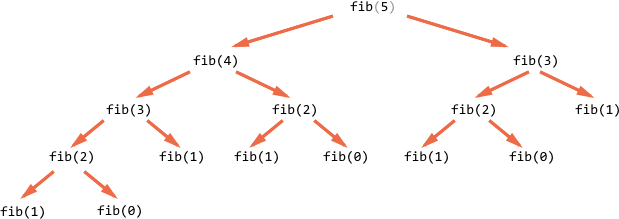
\includegraphics[width=0.40\textwidth]{figures/fibonacci-recursion-tree.png}
  \caption{A tree representing the recursive calls made to the Fibonacci function.}
  \label{fig:recursion}
\end{figure}

%second column
\begin{figure}[H]
  \centering
  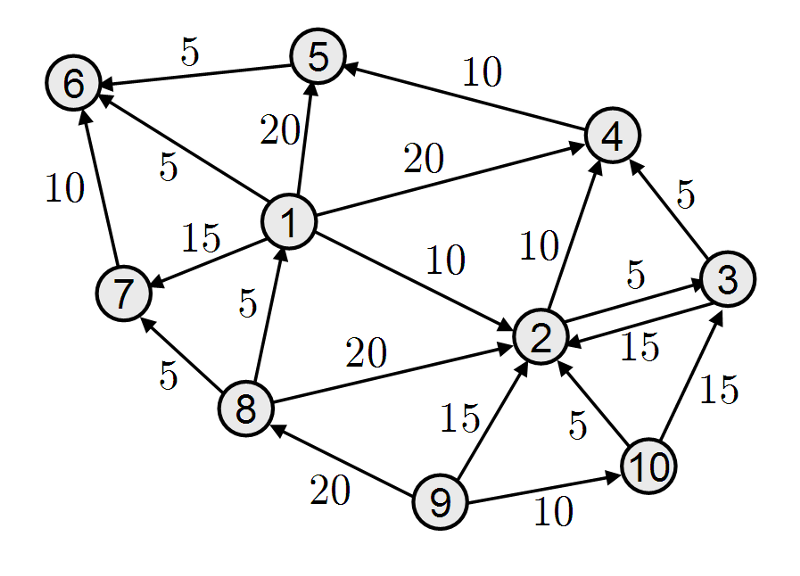
\includegraphics[width=0.20\textwidth]{figures/graph-theory.png}
  \caption{A graph theoretic representation of nodes, directed edges, and weights.}
  \label{fig:graph_theory}
\end{figure}
\end{multicols}

\section{Easy Problem}
\label{prob:easy}
Find $f(-1)$:
\begin{equation*}
f(x) =
\begin{cases}
x - f(x+1) & \text{if $x < 3$}\\
f(2x) & \text{if $3 \leq x < 5$}\\
x + 1 & otherwise
\end{cases}
\end{equation*}
\vspace{2cm}

\hfill
    \begin{tabular}[b]{|c|}
        \hline
        Your\\
        Answer:\\
        \\
        \hline
    \end{tabular}
\hfill

\section{Medium Problem}
\label{prob:medium}
Let $n$ be any positive base 10 integer from 1 to $2^{12}$ inclusive.
Let $S(n)$ be the number of 1's in the binary representation of $n$.
Find the number of possible $n$'s such that $S(n) - S(n + 1) = 3$.
\vspace{2cm}

\hfill
    \begin{tabular}[b]{|c|}
        \hline
        Your\\
        Answer:\\
        \\
        \hline
    \end{tabular}
\hfill

\section{Hard Problem}
\label{prob:hard}
Ackerman's function is defined as:

\begin{equation*}
A(x, y) =
\begin{cases}
y + 1 & \text{if $x = 0$}\\
A(x - 1, 1) & \text{if $x \neq 0$ and $y = 0$}\\
A(x - 1, A(x, y - 1)) & \text{if $x \neq 0$ and $y \neq 0$}
\end{cases}
\end{equation*}
Find $A(3, 4)$.
\vspace{2cm}

\hfill
    \begin{tabular}[b]{|c|}
        \hline
        Your\\
        Answer:\\
        \\
        \hline
    \end{tabular}
\hfill
\end{document}
